% ============================================================
\chapter{Artificial Neural Networks --- Foundations}
\label{ch:neural_networks}
% ============================================================

\begin{intuition}
An artificial neural network is a parametric function that learns to transform inputs into outputs by progressively adjusting its parameters. Like a child learning to recognize cats by seeing thousands of images, the network refines its internal representations with each example.
\end{intuition}

% ------------------------------------------------------------
\section{The Formal Neuron}
\label{sec:neuron}
\index{formal neuron}

\subsection{Mathematical Model}

The formal neuron, inspired by the McCulloch-Pitts model (1943), computes a weighted sum of its inputs followed by an activation function\index{activation function}:

\begin{mathbox}[title=\textbf{Formal Neuron}]
Let $\bm{x} = (x_1, \ldots, x_d)^\top \in \R^d$ be the input vector, $\bm{w} = (w_1, \ldots, w_d)^\top \in \R^d$ the weight vector, and $b \in \R$ the bias. The neuron's output is:
\[
y = \sigma\!\left(\sum_{i=1}^d w_i x_i + b\right) = \sigma(\bm{w}^\top \bm{x} + b)
\]
where $\sigma : \R \to \R$ is the activation function.
\end{mathbox}

\begin{center}
\begin{tikzpicture}[
    neuron/.style={circle, draw=NavyBlue, thick, minimum size=1.2cm, fill=blue!10},
    input/.style={circle, draw=gray, thick, minimum size=0.8cm, fill=gray!10},
    >=Stealth
]
\foreach \i/\lab in {1/$x_1$, 2/$x_2$, 3/$x_d$} {
    \node[input] (x\i) at (0, -\i*1.5+1.5) {\lab};
}
\node at (0, -1.5) {$\vdots$};
\node[neuron] (n) at (4, -0.75) {$\sum$, $\sigma$};
\node[right=1.5cm of n] (y) {$y$};
\foreach \i/\w in {1/$w_1$, 2/$w_2$, 3/$w_d$} {
    \draw[->, thick] (x\i) -- node[above, sloped, font=\small] {\w} (n);
}
\node[above=0.5cm of n, font=\small] (b) {$b$};
\draw[->, thick] (b) -- (n);
\draw[->, thick] (n) -- (y);
\end{tikzpicture}
\end{center}

\subsection{Activation Functions}
\index{activation function!sigmoid}
\index{activation function!ReLU}
\index{activation function!tanh}

Activation functions introduce the nonlinearity essential to the network's expressive power:

\begin{center}
\begin{tabular}{llll}
\toprule
\textbf{Name} & \textbf{Formula} & \textbf{Range} & \textbf{Usage} \\
\midrule
Sigmoid & $\sigma(z) = \frac{1}{1+e^{-z}}$ & $(0,1)$ & Binary output \\[6pt]
Tanh & $\tanh(z) = \frac{e^z - e^{-z}}{e^z + e^{-z}}$ & $(-1,1)$ & Hidden layers (historical) \\[6pt]
ReLU & $\relu(z) = \max(0,z)$ & $[0,+\infty)$ & Modern standard \\[6pt]
Leaky ReLU & $\max(\alpha z, z)$, $\alpha\approx 0.01$ & $\R$ & Avoids dead neurons \\[6pt]
GELU & $z \cdot \Phi(z)$ & $\R$ & Transformers \\[6pt]
Softmax & $\frac{e^{z_i}}{\sum_j e^{z_j}}$ & $(0,1)^K$ & Multi-class classification \\
\bottomrule
\end{tabular}
\end{center}

\begin{center}
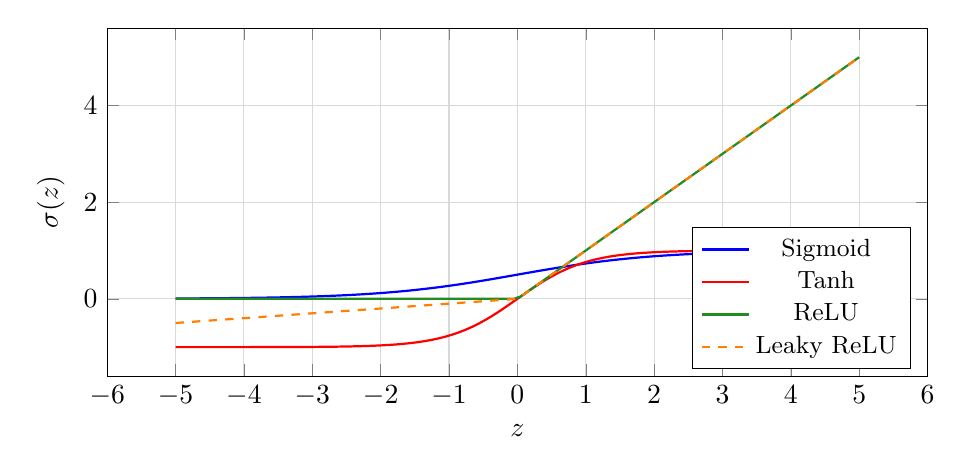
\begin{tikzpicture}
\begin{axis}[
    width=12cm, height=6cm,
    xlabel={$z$}, ylabel={$\sigma(z)$},
    domain=-5:5, samples=100,
    legend style={at={(0.98,0.02)}, anchor=south east, font=\small},
    grid=major, grid style={gray!30}
]
\addplot[blue, thick] {1/(1+exp(-x))}; \addlegendentry{Sigmoid}
\addplot[red, thick] {tanh(x)}; \addlegendentry{Tanh}
\addplot[ForestGreen, thick] {max(0,x)}; \addlegendentry{ReLU}
\addplot[orange, thick, dashed] {x > 0 ? x : 0.1*x}; \addlegendentry{Leaky ReLU}
\end{axis}
\end{tikzpicture}
\end{center}

\begin{warning}
The sigmoid suffers from the \textbf{vanishing gradient}\index{vanishing gradient} problem: for $|z| \gg 0$, $\sigma'(z) \approx 0$, which stalls learning in deep layers. This is why ReLU is now the default choice.
\end{warning}

% ------------------------------------------------------------
\section{Multilayer Perceptron (MLP)}
\label{sec:mlp}
\index{multilayer perceptron}
\index{MLP|see{multilayer perceptron}}

\subsection{Architecture}

A multilayer perceptron stacks $L$ layers of neurons. Layer $\ell$ performs:
\[
\bm{h}^{(\ell)} = \sigma^{(\ell)}\!\left(W^{(\ell)} \bm{h}^{(\ell-1)} + \bm{b}^{(\ell)}\right), \quad \ell = 1, \ldots, L
\]
where $\bm{h}^{(0)} = \bm{x}$ is the input and $\bm{h}^{(L)} = \hat{\bm{y}}$ is the output.

\begin{definition}[Fully Connected Network]
\label{def:fc}
An MLP with $L$ layers of widths $n_0, n_1, \ldots, n_L$ is the composition:
\[
f_\theta(\bm{x}) = \sigma^{(L)} \circ A^{(L)} \circ \sigma^{(L-1)} \circ A^{(L-1)} \circ \cdots \circ \sigma^{(1)} \circ A^{(1)}(\bm{x})
\]
where $A^{(\ell)}(\bm{z}) = W^{(\ell)}\bm{z} + \bm{b}^{(\ell)}$ is an affine transformation with $W^{(\ell)} \in \R^{n_\ell \times n_{\ell-1}}$, and $\theta = \{W^{(\ell)}, \bm{b}^{(\ell)}\}_{\ell=1}^L$ denotes the full parameter set.
\end{definition}

\begin{center}
\begin{tikzpicture}[
    neuron/.style={circle, draw=NavyBlue, thick, minimum size=0.7cm, fill=blue!10},
    inputn/.style={circle, draw=ForestGreen, thick, minimum size=0.7cm, fill=green!10},
    outputn/.style={circle, draw=BrickRed, thick, minimum size=0.7cm, fill=red!10},
    >=Stealth
]
\foreach \i in {1,...,4} {
    \node[inputn] (i\i) at (0, -\i*1.2+3) {};
}
\node[below=0.1cm of i4, font=\small, ForestGreen] {Input};
\foreach \i in {1,...,5} {
    \node[neuron] (h1\i) at (3, -\i*1.0+3) {};
}
\node[below=0.1cm of h15, font=\small, NavyBlue] {Layer 1};
\foreach \i in {1,...,5} {
    \node[neuron] (h2\i) at (6, -\i*1.0+3) {};
}
\node[below=0.1cm of h25, font=\small, NavyBlue] {Layer 2};
\foreach \i in {1,...,3} {
    \node[outputn] (o\i) at (9, -\i*1.2+2.4) {};
}
\node[below=0.1cm of o3, font=\small, BrickRed] {Output};
\foreach \i in {1,...,4} {
    \foreach \j in {1,...,5} {
        \draw[gray!40] (i\i) -- (h1\j);
    }
}
\foreach \i in {1,...,5} {
    \foreach \j in {1,...,5} {
        \draw[gray!40] (h1\i) -- (h2\j);
    }
}
\foreach \i in {1,...,5} {
    \foreach \j in {1,...,3} {
        \draw[gray!40] (h2\i) -- (o\j);
    }
}
\end{tikzpicture}
\end{center}

\subsection{Parameter Count}

For an MLP with layers $(n_0, n_1, \ldots, n_L)$, the total number of parameters is:
\[
|\theta| = \sum_{\ell=1}^{L} (n_{\ell-1} \cdot n_\ell + n_\ell) = \sum_{\ell=1}^{L} n_\ell(n_{\ell-1} + 1)
\]

\begin{example}
An MLP $(784, 256, 128, 10)$ for MNIST has $784 \times 256 + 256 + 256 \times 128 + 128 + 128 \times 10 + 10 = 235{,}146$ parameters.
\end{example}

% ------------------------------------------------------------
\section{Loss Functions}
\label{sec:loss}
\index{loss function}

\subsection{Regression: Mean Squared Error}
\index{MSE|see{mean squared error}}

For regression, we minimize the mean squared error (MSE):
\[
\mathcal{L}_{\mathrm{MSE}}(\theta) = \frac{1}{N} \sum_{i=1}^{N} \|\bm{y}_i - f_\theta(\bm{x}_i)\|^2
\]

\subsection{Classification: Cross-Entropy}
\index{cross-entropy}

For $K$-class classification with softmax output:
\[
\mathcal{L}_{\mathrm{CE}}(\theta) = -\frac{1}{N}\sum_{i=1}^{N} \sum_{k=1}^{K} y_{ik} \log \hat{y}_{ik}
\]
where $y_{ik} \in \{0,1\}$ is the one-hot encoding and $\hat{y}_{ik} = \softmax(z_{ik})$.

\begin{mathbox}[title=\textbf{Connection to Maximum Likelihood}]
Minimizing cross-entropy is equivalent to maximizing the log-likelihood under a categorical model:
\[
\hat{\theta}_{\mathrm{MLE}} = \argmax_\theta \sum_{i=1}^N \log p(y_i \mid \bm{x}_i; \theta) = \argmin_\theta \mathcal{L}_{\mathrm{CE}}(\theta)
\]
\end{mathbox}

\subsection{Binary Classification: Binary Cross-Entropy}
\index{cross-entropy!binary}

For $K=2$ with sigmoid output:
\[
\mathcal{L}_{\mathrm{BCE}}(\theta) = -\frac{1}{N}\sum_{i=1}^{N} \left[y_i \log \hat{y}_i + (1-y_i)\log(1-\hat{y}_i)\right]
\]

% ------------------------------------------------------------
\section{Universal Approximation Theorem}
\label{sec:uat}
\index{universal approximation}

\begin{theorem}[Cybenko, 1989; Hornik, 1991]
\label{thm:uat}
Let $\sigma$ be a continuous, non-polynomial activation function. For any continuous function $f : [0,1]^d \to \R$ and any $\varepsilon > 0$, there exist $n \in \N$, weights $w_{ij}, b_j, c_j$ such that:
\[
\left| f(\bm{x}) - \sum_{j=1}^{n} c_j \, \sigma\!\left(\sum_{i=1}^d w_{ij} x_i + b_j\right) \right| < \varepsilon \quad \forall \bm{x} \in [0,1]^d
\]
\end{theorem}

\begin{intuition}
The universal approximation theorem states that a single hidden layer MLP of \emph{sufficient width} can approximate any continuous function. However, it says nothing about:
\begin{itemize}
\item The \textbf{width} $n$ required (which can be exponentially large).
\item The \textbf{ease of learning} the optimal weights.
\item The advantage of \textbf{depth} (multiple layers) over width.
\end{itemize}
In practice, deep networks achieve better performance with far fewer parameters than wide, shallow networks.
\end{intuition}

% ------------------------------------------------------------
\section{Weight Initialization}
\label{sec:init}
\index{weight initialization}
\index{Xavier|see{weight initialization}}
\index{He|see{weight initialization}}

Poor initialization can cause activation explosion or vanishing from the very first forward pass.

\begin{mathbox}[title=\textbf{Xavier/Glorot Initialization (2010)}]
To preserve activation variance across layers with symmetric activations (tanh, linear sigmoid):
\[
W^{(\ell)}_{ij} \sim \mathcal{U}\!\left(-\sqrt{\frac{6}{n_{\ell-1}+n_\ell}}, \sqrt{\frac{6}{n_{\ell-1}+n_\ell}}\right)
\]
\end{mathbox}

\begin{mathbox}[title=\textbf{He/Kaiming Initialization (2015)}]
For ReLU activations (which zero out half the activations):
\[
W^{(\ell)}_{ij} \sim \mathcal{N}\!\left(0, \frac{2}{n_{\ell-1}}\right)
\]
\end{mathbox}

% ------------------------------------------------------------
\section{PyTorch Implementation}
\label{sec:impl_mlp}

\begin{codeblock}[title=\textbf{MLP in PyTorch --- MNIST Classification}]
\begin{minted}{python}
import torch
import torch.nn as nn
import torch.optim as optim
from torchvision import datasets, transforms
from torch.utils.data import DataLoader

# Hyperparameters
BATCH_SIZE = 128
LR = 1e-3
EPOCHS = 10
DEVICE = torch.device('cuda' if torch.cuda.is_available() else 'cpu')

# MNIST data
transform = transforms.Compose([
    transforms.ToTensor(),
    transforms.Normalize((0.1307,), (0.3081,))
])
train_data = datasets.MNIST('./data', train=True, download=True,
                            transform=transform)
test_data = datasets.MNIST('./data', train=False, transform=transform)
train_loader = DataLoader(train_data, batch_size=BATCH_SIZE, shuffle=True)
test_loader = DataLoader(test_data, batch_size=BATCH_SIZE)

# MLP model
class MLP(nn.Module):
    def __init__(self, input_dim=784, hidden_dims=[256, 128],
                 num_classes=10):
        super().__init__()
        layers = []
        prev = input_dim
        for h in hidden_dims:
            layers += [nn.Linear(prev, h), nn.ReLU()]
            prev = h
        layers.append(nn.Linear(prev, num_classes))
        self.net = nn.Sequential(*layers)

    def forward(self, x):
        return self.net(x.view(x.size(0), -1))  # Flatten

model = MLP().to(DEVICE)
print(f"Parameters: {sum(p.numel() for p in model.parameters()):,}")

# Training
criterion = nn.CrossEntropyLoss()
optimizer = optim.Adam(model.parameters(), lr=LR)

for epoch in range(1, EPOCHS + 1):
    model.train()
    total_loss = 0
    for X, y in train_loader:
        X, y = X.to(DEVICE), y.to(DEVICE)
        optimizer.zero_grad()
        loss = criterion(model(X), y)
        loss.backward()
        optimizer.step()
        total_loss += loss.item() * X.size(0)

    # Evaluation
    model.eval()
    correct = 0
    with torch.no_grad():
        for X, y in test_loader:
            X, y = X.to(DEVICE), y.to(DEVICE)
            correct += (model(X).argmax(1) == y).sum().item()

    acc = correct / len(test_data)
    print(f"Epoch {epoch:2d} | Loss: {total_loss/len(train_data):.4f}"
          f" | Test Acc: {acc:.4f}")
\end{minted}
\end{codeblock}

\begin{codeoutput}
\begin{verbatim}
Parameters: 235,146
Epoch  1 | Loss: 0.2534 | Test Acc: 0.9612
Epoch  2 | Loss: 0.1042 | Test Acc: 0.9710
...
Epoch 10 | Loss: 0.0198 | Test Acc: 0.9793
\end{verbatim}
\end{codeoutput}

% ------------------------------------------------------------
\section{Ablation Study: Width and Depth}
\label{sec:ablation_mlp}

\begin{codeblock}[title=\textbf{Ablation Study}]
\begin{minted}{python}
configs = {
    "Shallow-wide":  [1024],
    "2-layers":      [256, 128],
    "3-layers":      [256, 128, 64],
    "Deep-narrow":   [64, 64, 64, 64],
}

results = {}
for name, hidden in configs.items():
    model = MLP(hidden_dims=hidden).to(DEVICE)
    n_params = sum(p.numel() for p in model.parameters())
    # ... train and evaluate ...
    results[name] = {"params": n_params, "acc": test_acc}
    print(f"{name:20s} | {n_params:>8,} params | Acc: {test_acc:.4f}")
\end{minted}
\end{codeblock}

\begin{codeoutput}
\begin{verbatim}
Shallow-wide         |  812,042 params | Acc: 0.9781
2-layers             |  235,146 params | Acc: 0.9793
3-layers             |  243,338 params | Acc: 0.9802
Deep-narrow          |   63,434 params | Acc: 0.9745
\end{verbatim}
\end{codeoutput}

\begin{remark}
The 3-layer architecture achieves the best accuracy with a reasonable parameter count. The wide shallow network uses $3\times$ more parameters for a similar result. The deep narrow network, while economical, loses performance --- minimum width per layer matters.
\end{remark}

% ------------------------------------------------------------
\section{Connection to the State of the Art}
\label{sec:sota_mlp}

\begin{sota}
\begin{itemize}
\item \textbf{MLP-Mixer} (Tolstikhin et al., 2021): a purely MLP architecture for vision, rivaling CNNs and ViTs using only token-mixing and channel-mixing layers.
\item \textbf{KAN} (Kolmogorov-Arnold Networks, Liu et al., 2024): replace fixed weights with learnable functions on edges, improving interpretability and efficiency on scientific problems.
\item \textbf{Scaling laws} (Kaplan et al., 2020): network performance follows power laws as a function of parameter count, dataset size, and compute budget.
\end{itemize}
\end{sota}

% ------------------------------------------------------------
\section{Chapter Summary}

\begin{keyformulas}
\begin{itemize}
\item \textbf{Formal neuron}: $y = \sigma(\bm{w}^\top \bm{x} + b)$
\item \textbf{MLP}: $f_\theta = \sigma^{(L)} \circ A^{(L)} \circ \cdots \circ \sigma^{(1)} \circ A^{(1)}$
\item \textbf{MSE loss}: $\frac{1}{N}\sum_i \|y_i - \hat{y}_i\|^2$
\item \textbf{CE loss}: $-\frac{1}{N}\sum_i \sum_k y_{ik}\log\hat{y}_{ik}$
\item \textbf{Xavier init}: $W \sim \mathcal{U}(-\sqrt{6/(n_{\mathrm{in}}+n_{\mathrm{out}})}, +\cdot)$
\item \textbf{He init}: $W \sim \mathcal{N}(0, 2/n_{\mathrm{in}})$
\item \textbf{UAT}: a single hidden layer MLP can approximate any continuous function
\end{itemize}
\end{keyformulas}

% ------------------------------------------------------------
\section{Exercises}

\begin{exercise}[$\star$ --- Derivation]
Show that the derivative of the sigmoid satisfies $\sigma'(z) = \sigma(z)(1 - \sigma(z))$. Deduce that $\max_z \sigma'(z) = 1/4$.
\end{exercise}

\begin{exercise}[$\star$ --- Parameter Counting]
Compute the exact number of parameters in an MLP $(1024, 512, 256, 128, 10)$. Compare with a network $(1024, 2048, 10)$ of approximately the same parameter budget.
\end{exercise}

\begin{exercise}[$\star\star$ --- Implementation]
Implement an MLP in PyTorch for Fashion-MNIST classification (10 clothing classes). Compare performance with ReLU, Leaky ReLU, and GELU. Plot the learning curves.
\end{exercise}

\begin{exercise}[$\star\star$ --- Ablation Study]
Conduct a systematic ablation study on MNIST varying: (a) the number of layers from 1 to 6, (b) the width from 32 to 512. Plot a heatmap of accuracy vs (depth, width).
\end{exercise}

\begin{exercise}[$\star\star\star$ --- Research Project]
Implement an MLP-Mixer for CIFAR-10 following Tolstikhin et al. (2021). Compare its performance with a standard MLP and a simple CNN. Analyze the influence of patch size and hidden dimension.
\end{exercise}
